% =====================================================================
%  Assessment 1 -- Objective 1: longitudinal and lateral dynamics of the
%  MR2006B differential-drive vehicle, identified by least squares.
%  IEEEtran if installed, IEEE-style two-column fallback otherwise.
%  Red [bracketed] text = items the team still has to supply.
%  Numbers come from results.tex / cv_table.tex (MATLAB), never typed here.
% =====================================================================
\IfFileExists{IEEEtran.cls}{%
  \documentclass[conference]{IEEEtran}\newcommand{\haveieee}{}%
}{%
  \documentclass[10pt,twocolumn,letterpaper]{article}%
}
\usepackage[T1]{fontenc}
\usepackage[utf8]{inputenc}
\usepackage{amsmath,amssymb}
\usepackage{booktabs,catchfile,array,graphicx,xcolor,cite,balance,microtype}
\usepackage{tikz}
\usetikzlibrary{shapes.geometric,arrows.meta,positioning,calc,fit,backgrounds}

\makeatletter
\@ifundefined{haveieee}{%
  \usepackage{mathptmx}
  \usepackage[letterpaper,top=0.75in,bottom=0.9in,left=0.625in,right=0.625in,columnsep=0.25in]{geometry}
  \usepackage{titlesec}
  \usepackage{caption}
  \renewcommand\thesection{\Roman{section}}
  \renewcommand\thesubsection{\Alph{subsection}}
  \titleformat{\section}[block]{\centering\small\scshape}{\thesection.}{0.5em}{}
  \titleformat{\subsection}[block]{\itshape\small}{\thesubsection.}{0.5em}{}
  \titlespacing*{\section}{0pt}{1.2ex plus .3ex}{0.8ex}
  \titlespacing*{\subsection}{0pt}{1ex plus .3ex}{0.5ex}
  \setlength{\parskip}{0pt}
  \captionsetup[figure]{name={Fig.},labelsep=period,font=footnotesize}
  \captionsetup[table]{name=TABLE,labelsep=newline,font=footnotesize,textfont=sc,justification=centering,singlelinecheck=off}
  \renewcommand{\thetable}{\Roman{table}}
  \renewenvironment{abstract}{\noindent\small\bfseries\itshape Abstract\upshape---}{\par\vspace{0.6ex}\normalfont}
  \newenvironment{IEEEkeywords}{\noindent\small\bfseries\itshape Keywords\upshape---\itshape}{\par\vspace{0.6ex}\normalfont}
  \newcommand{\IEEEauthorblockN}[1]{\normalsize #1\\[0.3ex]}
  \newcommand{\IEEEauthorblockA}[1]{\small\itshape #1}
  \renewcommand{\@maketitle}{\newpage\null\vskip 1ex
    \begin{center}{\fontsize{22}{24}\selectfont \@title\par}\vskip 2ex
      {\lineskip .5em\begin{tabular}[t]{c}\@author\end{tabular}\par}\end{center}\par\vskip 1ex}
}{}
\makeatother

\newcommand{\todo}[1]{{\color{red}\textbf{[#1]}}}
\setlength{\textfloatsep}{8pt plus 2pt minus 2pt}
\setlength{\floatsep}{8pt plus 2pt minus 2pt}
\setlength{\intextsep}{8pt plus 2pt minus 2pt}

\tikzset{
  blk/.style={draw=black!70,fill=green!8,rounded corners=1.5pt,minimum height=0.7cm,align=center,font=\scriptsize,inner sep=2pt},
  hw/.style={blk,fill=orange!10},
  arr/.style={-{Stealth[length=1.8mm]},thick},
  lb/.style={font=\tiny,inner sep=1pt}
}

% ---- results from MATLAB; every macro has a visible fallback ----------
\IfFileExists{results.tex}{% generated by run_assessment1.m
\newcommand{\DataSource}{experimental}
\newcommand{\TsMs}{20}
\newcommand{\LonA}{0.7416}
\newcommand{\LonB}{0.1680}
\newcommand{\LonC}{0.0000}
\newcommand{\LonDelay}{0}
\newcommand{\LonTauMs}{67}
\newcommand{\LonK}{0.650}
\newcommand{\LatA}{0.7554}
\newcommand{\LatB}{1.4206}
\newcommand{\LatE}{0.0635}
\newcommand{\LatDelay}{0}
\newcommand{\LatTauMs}{71}
\newcommand{\LatK}{5.81}
\newcommand{\RtwoLonTrain}{0.963}
\newcommand{\RtwoLonValStep}{0.988}
\newcommand{\RtwoLonValSine}{0.988}
\newcommand{\RtwoLatTrain}{0.985}
\newcommand{\RtwoLatVal}{0.987}
\newcommand{\RtwoLonArxTwoVal}{0.988}
\newcommand{\VquantMms}{3.18}
\newcommand{\LatKcheck}{5.83}
\newcommand{\LatKcheckPct}{\ensuremath{-}0.3}
\newcommand{\TsOverTauLon}{0.30}
\newcommand{\TsOverTauLat}{0.28}
}{}
\providecommand{\DataSource}{\todo{?}}
\providecommand{\TsMs}{20}
\newcommand{\fallbackmacros}{\todo{?}}
\providecommand{\LonA}{\fallbackmacros}\providecommand{\LonB}{\fallbackmacros}
\providecommand{\LonC}{\fallbackmacros}\providecommand{\LonDelay}{\fallbackmacros}
\providecommand{\LonTauMs}{\fallbackmacros}\providecommand{\LonK}{\fallbackmacros}
\providecommand{\LatA}{\fallbackmacros}\providecommand{\LatB}{\fallbackmacros}
\providecommand{\LatDelay}{\fallbackmacros}\providecommand{\LatTauMs}{\fallbackmacros}
\providecommand{\LatK}{\fallbackmacros}
\providecommand{\RtwoLonTrain}{\fallbackmacros}\providecommand{\RtwoLonValStep}{\fallbackmacros}
\providecommand{\RtwoLonValSine}{\fallbackmacros}\providecommand{\RtwoLatTrain}{\fallbackmacros}
\providecommand{\RtwoLatVal}{\fallbackmacros}\providecommand{\RtwoLonArxTwoVal}{\fallbackmacros}
\providecommand{\VquantMms}{\fallbackmacros}
\providecommand{\TsOverTauLon}{\fallbackmacros}\providecommand{\TsOverTauLat}{\fallbackmacros}

\IfFileExists{cv_table.tex}{\CatchFileDef{\cvrows}{cv_table.tex}{}}{\newcommand{\cvrows}{\todo{run MATLAB}\\}}
\def\synth{synthetic}
\newcommand{\synthnote}{\ifx\DataSource\synth
  {\color{red}\textbf{NOTE: all identified values, $R^2$ figures and plots in this version come from the \emph{synthetic} validation of the identification pipeline (simulated plant, known ground truth). They must be replaced by the experimental run before submission.}}\fi}

% figure with fallback box
\newcommand{\figorbox}[3][\linewidth]{\IfFileExists{#2}{\includegraphics[width=#1]{#2}}{%
  \fbox{\parbox[c][2.2cm][c]{0.85\linewidth}{\centering\todo{#3}\\[2pt]{\scriptsize\detokenize{#2}}}}}}
\newcommand{\pic}[2]{\IfFileExists{#1}{\includegraphics[width=\linewidth]{#1}}{%
  \fbox{\parbox[c][2.4cm][c]{0.85\linewidth}{\centering\todo{photo: #2}}}}}

\begin{document}

\title{Least-Squares Identification and Validation of the Longitudinal and Lateral Dynamics of a Differential-Drive Ground Vehicle}

\author{%
\IEEEauthorblockN{\todo{Author 1}}\IEEEauthorblockA{\todo{Affiliation, ID}}
\and
\IEEEauthorblockN{\todo{Author 2}}\IEEEauthorblockA{\todo{Affiliation, ID}}
\and
\IEEEauthorblockN{\todo{Author 3}}\IEEEauthorblockA{\todo{Affiliation, ID}}
\and
\IEEEauthorblockN{\todo{Author 4}}\IEEEauthorblockA{\todo{Affiliation, ID}}
}
\maketitle

\begin{abstract}
We identify the longitudinal (speed) and lateral (yaw-rate) dynamics of the MR2006B differential-drive vehicle from input--output experiments. The vehicle is driven by two brushed-DC gearmotors through BTS7960 drivers and controlled by an STM32F446 sampling at $T_s=\TsMs$~ms. Speed and yaw rate are reconstructed from the wheel encoders. Physical reasoning gives first-order models; their discrete parameters are estimated by ordinary least squares from a PRBS (longitudinal) and a double lane change (lateral), cross-validated on step and chirp tests and on a single lane change, and compared with a second-order ARX structure. Free-run simulation against held-out data gives $R^2=\RtwoLonValStep$ and $\RtwoLonValSine$ (longitudinal, step and chirp) and $R^2=\RtwoLatVal$ (lateral). The identified time constants are $\tau_\mathrm{lon}=\LonTauMs$~ms and $\tau_\mathrm{lat}=\LatTauMs$~ms. The sampling period, the quantisation of encoder speed and the absence of an IMU are discussed as limitations. \synthnote
\end{abstract}

\begin{IEEEkeywords}
system identification, least squares, differential drive, STM32, vehicle dynamics, cross-validation
\end{IEEEkeywords}

\section{Introduction}
Controller design for a ground vehicle needs a dynamic model that is accurate in the bandwidth of the loop, yet simple enough to identify from a few minutes of data. Classical vehicle-dynamics texts derive longitudinal and lateral models from first principles~\cite{rajamani2011,gillespie1992}; the parameters (inertia, friction, actuator gain) are then fitted to experiments with the methods of system identification~\cite{ljung1999}. For small differential-drive robots the kinematics are standard~\cite{siegwart2011}, but the dynamics that matter for the speed and steering loops, i.e.\ motor, driver and mass, must be measured.

This paper addresses Objective~1 of the course assessment: model the longitudinal and lateral dynamics of the vehicle by least squares (LS) with at least two experiments per axis, cross-validate on data not used for training, and report $R^2$ of the simulated against the measured response. Because the vehicle has no steering linkage, ``steering'' is the differential wheel command and the lateral response is the yaw rate. Section~II describes the hardware and justifies the sampling time, Section~III derives the models, Section~IV the estimator, Section~V the experiments, and Sections~VI--VII give results and limitations.

\section{System Description}
\subsection{Components and Roles}
Table~\ref{tab:comp} lists the components of the velocity and steering loops; Fig.~\ref{fig:blocks} shows the signal flow and Fig.~\ref{fig:wiring} the power and signal wiring (pin assignment from the firmware specification~\cite{fwspec}). Velocity and steering share the same actuators: the common duty $u=(u_L+u_R)/2$ sets speed and the differential duty $\delta=(u_R-u_L)/2$ sets yaw rate.

\begin{table}[!t]
\caption{Components of the velocity and steering loops}
\label{tab:comp}
\centering\footnotesize
\setlength{\tabcolsep}{2.5pt}
\begin{tabular}{@{}p{1.45cm}p{1.75cm}p{3.3cm}p{1.35cm}@{}}
\toprule
\textbf{Component} & \textbf{Part} & \textbf{Role} & \textbf{Interface}\\
\midrule
Controller & NUCLEO-F446RE (STM32F446RE, 180~MHz, FPU) & Tick, speed estimation, duty generation; runs the excitation profiles & --\\
PWM & TIM1, 20~kHz, 9000 steps & Actuator command $u_L,u_R$ & PA8--PA11\\
Driver & 2$\times$ BTS7960~\cite{bts7960} & Converts duty into mean motor voltage; both axes & PWM + EN (PB12/13)\\
Actuator & 2$\times$ JGB37-3530 gearmotor, 56.3:1 & Wheel torque: sum sets speed, difference sets yaw & H-bridge\\
Encoders & Hall, 64 counts/motor rev., TIM3 (L), TIM8 (R) & Wheel speeds, hence $v$ and $r$ & PA6/7, PC6/7\\
Battery sense & 3S LiPo, divider 47\,k/10\,k, ADC1 & Supply voltage (sag) & PA0\\
Radio / USB & HC-12 (USART1), ST-Link VCP (USART2) & Excitation start, log capture & PB6/7; PA2/3\\
\bottomrule
\end{tabular}
\end{table}

\begin{figure*}[!t]
\centering
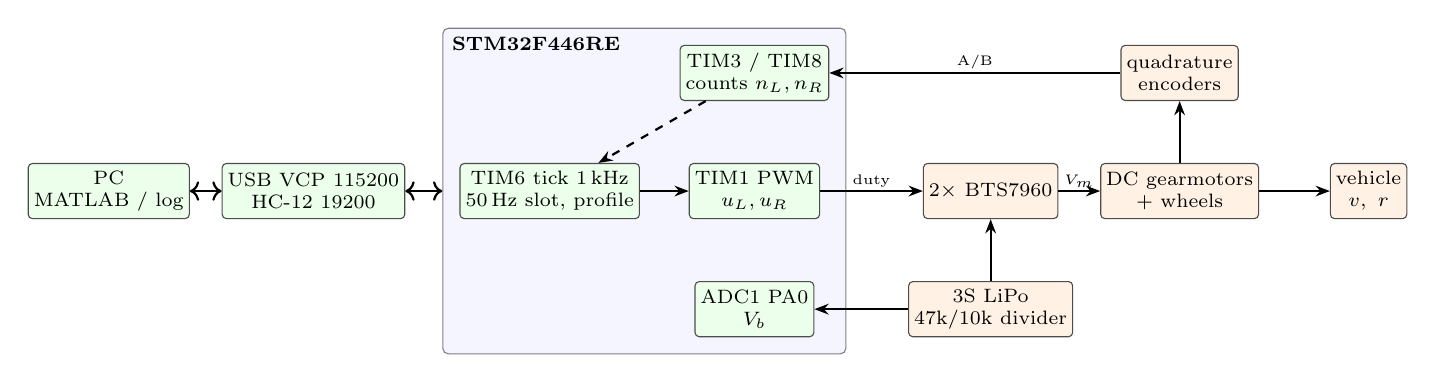
\begin{tikzpicture}[x=1cm,y=1cm]
\node[blk] (pc) at (0,0) {PC\\MATLAB / log};
\node[blk] (link) at (2.6,0) {USB VCP 115200\\HC-12 19200};
\node[blk] (tick) at (5.6,0.0) {TIM6 tick 1\,kHz\\50\,Hz slot, profile};
\node[blk] (pwm) at (8.2,0) {TIM1 PWM\\$u_L,u_R$};
\node[blk] (cnt) at (8.2,1.5) {TIM3 / TIM8\\counts $n_L,n_R$};
\node[blk] (adc) at (8.2,-1.5) {ADC1 PA0\\$V_b$};
\begin{scope}[on background layer]
\node[draw=black!50,fill=blue!4,rounded corners=2pt,fit=(tick)(pwm)(cnt)(adc),inner sep=6pt,label={[font=\scriptsize\bfseries,anchor=north west]north west:STM32F446RE}] (mcu) {};
\end{scope}
\node[hw] (drv) at (11.2,0) {2$\times$ BTS7960};
\node[hw] (mot) at (13.6,0) {DC gearmotors\\+ wheels};
\node[hw] (veh) at (16.0,0) {vehicle\\$v,\ r$};
\node[hw] (enc) at (13.6,1.5) {quadrature\\encoders};
\node[hw] (bat) at (11.2,-1.5) {3S LiPo\\47k/10k divider};
\draw[arr,<->] (pc) -- (link);
\draw[arr,<->] (link) -- (tick-|mcu.west);
\draw[arr] (tick) -- (pwm);
\draw[arr] (pwm) -- node[lb,above]{duty} (drv);
\draw[arr] (drv) -- node[lb,above]{$V_m$} (mot);
\draw[arr] (mot) -- (veh);
\draw[arr] (mot) -- (enc);
\draw[arr] (enc) -- node[lb,above]{A/B} (cnt);
\draw[arr] (bat) -- (adc);
\draw[arr] (bat) -- (drv);
\draw[arr,dashed] (cnt) -- (tick);
\end{tikzpicture}
\caption{Signal flow of the speed and steering loops. The PC starts the excitation; the firmware sets $u_L,u_R$ through TIM1 and the BTS7960 drivers; the encoders return counts per 20~ms, from which $v$ and $r$ are computed offline. The battery divider (ADC1) is not used in the identification.}
\label{fig:blocks}
\end{figure*}

\begin{figure*}[!t]
\centering
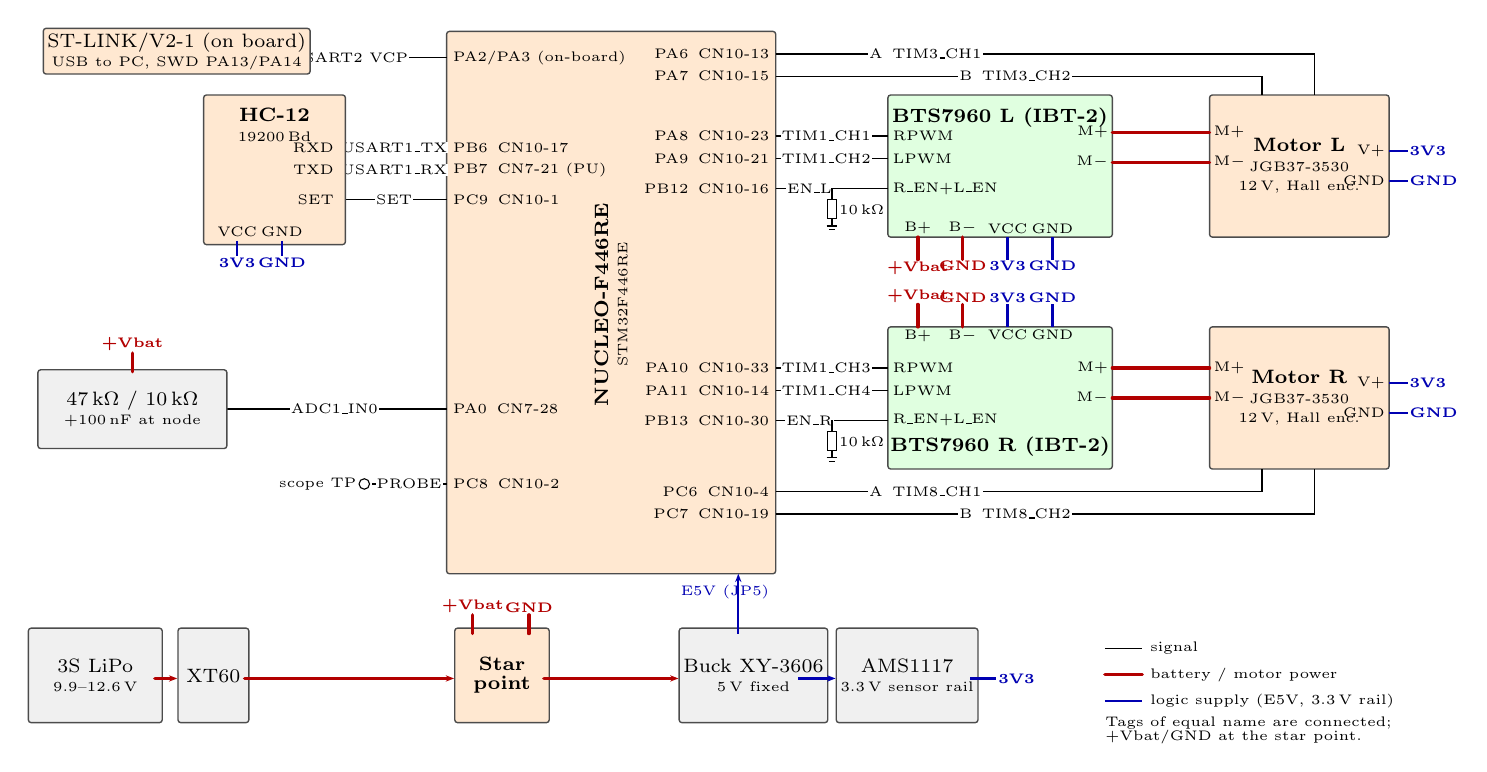
\begin{tikzpicture}[x=0.95cm,y=0.95cm,
  font=\scriptsize,
  wpow/.style={draw=red!70!black,very thick,line cap=round},
  wlog/.style={draw=blue!70!black,thick},
  wsig/.style={draw=black,line width=0.5pt},
  wl/.style={font=\tiny,fill=white,inner sep=0.4pt},
  pn/.style={font=\tiny,inner sep=0pt},
  bx/.style={draw=black!70,rounded corners=1pt,line width=0.5pt,align=center,inner sep=1.5pt},
  bsys/.style={bx,fill=green!12},
  bhw/.style={bx,fill=orange!18},
  bpw/.style={bx,fill=black!6},
  tgp/.style={font=\tiny\bfseries,red!70!black,inner sep=0.5pt},
  tgl/.style={font=\tiny\bfseries,blue!70!black,inner sep=0.5pt}]

\draw[bx,fill=orange!18,draw=black!70] (5.6,2.0) rectangle (10.0,9.25);
\node[rotate=90,align=center] at (7.8,5.6) {\textbf{NUCLEO-F446RE}\\[-1pt]\tiny STM32F446RE};
\node[pn,anchor=west] at (5.68,8.9) {PA2/PA3 (on-board)};
\draw[wsig] (5.6,8.9) -- (3.0,8.9) node[wl,pos=.5] {USART2 VCP};
\node[pn,anchor=west] at (5.68,7.7) {PB6 \,CN10-17};
\draw[wsig] (5.6,7.7) -- (4.2,7.7) node[wl,pos=.5] {USART1\_TX};
\node[pn,anchor=west] at (5.68,7.4) {PB7 \,CN7-21 (PU)};
\draw[wsig] (5.6,7.4) -- (4.2,7.4) node[wl,pos=.5] {USART1\_RX};
\node[pn,anchor=west] at (5.68,7.0) {PC9 \,CN10-1};
\draw[wsig] (5.6,7.0) -- (4.2,7.0) node[wl,pos=.5] {SET};
\node[pn,anchor=west] at (5.68,4.2) {PA0 \,CN7-28};
\draw[wsig] (5.6,4.2) -- (2.6,4.2) node[wl,pos=.5] {ADC1\_IN0};
\node[pn,anchor=west] at (5.68,3.2) {PC8 \,CN10-2};
\draw[wsig] (5.6,3.2) -- (4.6,3.2) node[wl,pos=.5] {PROBE};
\node[bhw,anchor=north west,minimum width=2.8cm] (stl) at (0.2,9.3) {ST-LINK/V2-1 (on board)\\[-1pt]\tiny USB to PC, SWD PA13/PA14};
\node[bhw,minimum width=1.8cm,minimum height=1.9cm] (hc) at (3.3,7.4) {};
\node[align=center] at (3.3,8.0) {\textbf{HC-12}\\[-1pt]\tiny 19200\,Bd};
\node[pn,anchor=east] at (4.1,7.7) {RXD};
\node[pn,anchor=east] at (4.1,7.4) {TXD};
\node[pn,anchor=east] at (4.1,7.0) {SET};
\node[pn,anchor=south] at (2.8,6.5) {VCC};
\draw[wlog] (2.8,6.45) -- (2.8,6.25); \node[tgl,anchor=north] at (2.8,6.25) {3V3};
\node[pn,anchor=south] at (3.4,6.5) {GND};
\draw[wlog] (3.4,6.45) -- (3.4,6.25); \node[tgl,anchor=north] at (3.4,6.25) {GND};
\node[bpw,minimum width=2.4cm,minimum height=1.0cm,align=center] (div) at (1.4,4.2) {47\,k$\Omega$ / 10\,k$\Omega$\\[-1pt]\tiny $+$100\,nF at node};
\draw[wpow] (1.4,4.7) -- (1.4,4.95); \node[tgp,anchor=south] at (1.4,4.95) {+Vbat};
\draw[fill=white,draw=black] (4.5,3.2) circle (0.07); \node[pn,anchor=east] at (4.4,3.2) {scope TP};
\draw[bx,fill=green!12] (11.5,6.5) rectangle (14.5,8.4);
\node[anchor=north] at (13.0,8.360000000000001) {\textbf{BTS7960 L (IBT-2)}};
\node[pn,anchor=west] at (11.56,7.85) {RPWM};
\node[pn,anchor=west] at (11.56,7.55) {LPWM};
\node[pn,anchor=west] at (11.56,7.15) {R\_EN+L\_EN};
\draw[bx,fill=green!12] (11.5,3.4) rectangle (14.5,5.3);
\node[anchor=south] at (13.0,3.44) {\textbf{BTS7960 R (IBT-2)}};
\node[pn,anchor=west] at (11.56,4.75) {RPWM};
\node[pn,anchor=west] at (11.56,4.45) {LPWM};
\node[pn,anchor=west] at (11.56,4.05) {R\_EN+L\_EN};
\node[pn,anchor=east] at (9.92,8.95) {PA6 \,CN10-13};
\node[pn,anchor=east] at (9.92,8.65) {PA7 \,CN10-15};
\node[pn,anchor=east] at (9.92,7.85) {PA8 \,CN10-23};
\node[pn,anchor=east] at (9.92,7.55) {PA9 \,CN10-21};
\node[pn,anchor=east] at (9.92,7.15) {PB12 \,CN10-16};
\node[pn,anchor=east] at (9.92,4.75) {PA10 \,CN10-33};
\node[pn,anchor=east] at (9.92,4.45) {PA11 \,CN10-14};
\node[pn,anchor=east] at (9.92,4.05) {PB13 \,CN10-30};
\node[pn,anchor=east] at (9.92,3.1) {PC6 \,CN10-4};
\node[pn,anchor=east] at (9.92,2.8) {PC7 \,CN10-19};
\draw[wsig] (10.0,7.85) -- (11.5,7.85) node[wl,pos=.45] {TIM1\_CH1};
\draw[wsig] (10.0,7.55) -- (11.5,7.55) node[wl,pos=.45] {TIM1\_CH2};
\draw[wsig] (10.0,4.75) -- (11.5,4.75) node[wl,pos=.45] {TIM1\_CH3};
\draw[wsig] (10.0,4.45) -- (11.5,4.45) node[wl,pos=.45] {TIM1\_CH4};
\draw[wsig] (10.0,7.15) -- (11.5,7.15) node[wl,pos=.3] {EN\_L};
\draw[wsig] (10.75,7.15) -- (10.75,7.0); \draw[fill=white,draw=black,line width=0.5pt] (10.69,7.0) rectangle (10.81,6.75);
\draw[wsig] (10.75,6.75) -- (10.75,6.65); \draw[wsig] (10.68,6.65) -- (10.82,6.65); \draw[wsig] (10.71,6.6000000000000005) -- (10.79,6.6000000000000005);
\node[pn,anchor=west] at (10.84,6.87) {10\,k$\Omega$};
\draw[wsig] (10.0,4.05) -- (11.5,4.05) node[wl,pos=.3] {EN\_R};
\draw[wsig] (10.75,4.05) -- (10.75,3.9); \draw[fill=white,draw=black,line width=0.5pt] (10.69,3.9) rectangle (10.81,3.65);
\draw[wsig] (10.75,3.65) -- (10.75,3.55); \draw[wsig] (10.68,3.55) -- (10.82,3.55); \draw[wsig] (10.71,3.5) -- (10.79,3.5);
\node[pn,anchor=west] at (10.84,3.7699999999999996) {10\,k$\Omega$};
\draw[bx,fill=orange!18] (15.8,6.5) rectangle (18.2,8.4);
\node[align=center] at (17.0,7.45) {\textbf{Motor L}\\[-1pt]\tiny JGB37-3530\\[-1pt]\tiny 12\,V, Hall enc.};
\draw[wpow] (14.5,7.9) -- (15.8,7.9);
\node[pn,anchor=east] at (14.45,7.9) {M+};
\node[pn,anchor=west] at (15.85,7.9) {M+};
\draw[wpow] (14.5,7.5) -- (15.8,7.5);
\node[pn,anchor=east] at (14.45,7.5) {M$-$};
\node[pn,anchor=west] at (15.85,7.5) {M$-$};
\draw[wsig] (10.0,8.95) -- (17.2,8.95) -- (17.2,8.4) node[pn,anchor=south west,inner sep=1pt,pos=0.0] {};
\draw[wsig] (10.0,8.65) -- (16.5,8.65) -- (16.5,8.4);
\node[wl] at (12.0,8.95) {A \,TIM3\_CH1};
\node[wl] at (13.2,8.65) {B \,TIM3\_CH2};
\node[pn,anchor=east] at (18.15,7.65) {V+};
\draw[wlog] (18.2,7.65) -- (18.45,7.65); \node[tgl,anchor=west] at (18.45,7.65) {3V3};
\node[pn,anchor=east] at (18.15,7.25) {GND};
\draw[wlog] (18.2,7.25) -- (18.45,7.25); \node[tgl,anchor=west] at (18.45,7.25) {GND};
\draw[bx,fill=orange!18] (15.8,3.4) rectangle (18.2,5.3);
\node[align=center] at (17.0,4.35) {\textbf{Motor R}\\[-1pt]\tiny JGB37-3530\\[-1pt]\tiny 12\,V, Hall enc.};
\draw[wpow] (14.5,4.75) -- (15.8,4.75);
\node[pn,anchor=east] at (14.45,4.75) {M+};
\node[pn,anchor=west] at (15.85,4.75) {M+};
\draw[wpow] (14.5,4.35) -- (15.8,4.35);
\node[pn,anchor=east] at (14.45,4.35) {M$-$};
\node[pn,anchor=west] at (15.85,4.35) {M$-$};
\draw[wsig] (10.0,3.1) -- (16.5,3.1) -- (16.5,3.4) node[pn,anchor=south west,inner sep=1pt,pos=0.0] {};
\draw[wsig] (10.0,2.8) -- (17.2,2.8) -- (17.2,3.4);
\node[wl] at (12.0,3.1) {A \,TIM8\_CH1};
\node[wl] at (13.2,2.8) {B \,TIM8\_CH2};
\node[pn,anchor=east] at (18.15,4.55) {V+};
\draw[wlog] (18.2,4.55) -- (18.45,4.55); \node[tgl,anchor=west] at (18.45,4.55) {3V3};
\node[pn,anchor=east] at (18.15,4.1499999999999995) {GND};
\draw[wlog] (18.2,4.1499999999999995) -- (18.45,4.1499999999999995); \node[tgl,anchor=west] at (18.45,4.1499999999999995) {GND};
\node[pn,anchor=south] at (11.9,6.54) {B+};
\draw[wpow] (11.9,6.5) -- (11.9,6.2);
\node[tgp,anchor=north] at (11.9,6.2) {+Vbat};
\node[pn,anchor=south] at (12.5,6.54) {B$-$};
\draw[wpow] (12.5,6.5) -- (12.5,6.2);
\node[tgp,anchor=north] at (12.5,6.2) {GND};
\node[pn,anchor=south] at (13.1,6.54) {VCC};
\draw[wlog] (13.1,6.5) -- (13.1,6.2);
\node[tgl,anchor=north] at (13.1,6.2) {3V3};
\node[pn,anchor=south] at (13.7,6.54) {GND};
\draw[wlog] (13.7,6.5) -- (13.7,6.2);
\node[tgl,anchor=north] at (13.7,6.2) {GND};
\node[pn,anchor=north] at (11.9,5.26) {B+};
\draw[wpow] (11.9,5.3) -- (11.9,5.6);
\node[tgp,anchor=south] at (11.9,5.6) {+Vbat};
\node[pn,anchor=north] at (12.5,5.26) {B$-$};
\draw[wpow] (12.5,5.3) -- (12.5,5.6);
\node[tgp,anchor=south] at (12.5,5.6) {GND};
\node[pn,anchor=north] at (13.1,5.26) {VCC};
\draw[wlog] (13.1,5.3) -- (13.1,5.6);
\node[tgl,anchor=south] at (13.1,5.6) {3V3};
\node[pn,anchor=north] at (13.7,5.26) {GND};
\draw[wlog] (13.7,5.3) -- (13.7,5.6);
\node[tgl,anchor=south] at (13.7,5.6) {GND};
\node[bpw,minimum width=1.7cm,minimum height=1.2cm,anchor=south west] at (0.0,0.0) {3S LiPo\\[-1pt]\tiny 9.9--12.6\,V};
\node[bpw,minimum width=0.8999999999999999cm,minimum height=1.2cm,anchor=south west] at (2.0,0.0) {XT60};
\node[bhw,minimum width=1.2000000000000002cm,minimum height=1.2cm,anchor=south west] at (5.7,0.0) {\textbf{Star}\\[-1pt]\textbf{point}};
\node[bpw,minimum width=1.6000000000000014cm,minimum height=1.2cm,anchor=south west] at (8.7,0.0) {Buck XY-3606\\[-1pt]\tiny 5\,V fixed};
\node[bpw,minimum width=1.799999999999999cm,minimum height=1.2cm,anchor=south west] at (10.8,0.0) {AMS1117\\[-1pt]\tiny 3.3\,V sensor rail};
\draw[wpow,-{Stealth[length=3pt]}] (1.7,0.6) -- (2.0,0.6);
\draw[wpow,-{Stealth[length=3pt]}] (2.9,0.6) -- (5.7,0.6);
\draw[wpow,-{Stealth[length=3pt]}] (6.9,0.6) -- (8.7,0.6);
\draw[wlog,-{Stealth[length=3pt]}] (10.3,0.6) -- (10.8,0.6);
\draw[wlog,-{Stealth[length=3pt]}] (9.5,1.2) -- (9.5,2.0);
\node[pn,anchor=east,blue!70!black] at (9.92,1.75) {E5V (JP5)};
\draw[wlog] (12.6,0.6) -- (12.95,0.6); \node[tgl,anchor=west] at (12.95,0.6) {3V3};
\draw[wpow] (5.95,1.2) -- (5.95,1.45); \node[tgp,anchor=south] at (5.95,1.45) {+Vbat};
\draw[wpow] (6.7,1.2) -- (6.7,1.45); \node[tgp,anchor=south] at (6.7,1.45) {GND};
\draw[wsig] (14.4,1.0) -- (14.9,1.0); \node[pn,anchor=west] at (15.0,1.0) {signal};
\draw[wpow] (14.4,0.65) -- (14.9,0.65); \node[pn,anchor=west] at (15.0,0.65) {battery / motor power};
\draw[wlog] (14.4,0.3) -- (14.9,0.3); \node[pn,anchor=west] at (15.0,0.3) {logic supply (E5V, 3.3\,V rail)};
\node[pn,anchor=west,align=left] at (14.4,-0.1) {Tags of equal name are connected;\\[-1pt] +Vbat/GND at the star point.};
\end{tikzpicture}

\caption{Wiring of the vehicle as built: NUCLEO-F446RE with two BTS7960 half-bridge modules driving the JGB37-3530 gearmotors (TIM1 PWM, EN lines with 10~k$\Omega$ pull-downs, TIM3/TIM8 quadrature encoders), HC-12 radio on USART1, ST-LINK console on USART2 and the battery divider on PA0. Power runs from the 3S LiPo through fuse and switch to a star point that feeds the drivers directly and, through a 5~V buck converter, the Nucleo (E5V) and the 3.3~V sensor rail. Pin assignment from the firmware specification~\cite{fwspec}.}
\label{fig:wiring}
\end{figure*}

\begin{figure}[!t]
\centering
\begin{minipage}{0.48\linewidth}\pic{figures/photo_vehicle.jpg}{vehicle top view}\end{minipage}\hfill
\begin{minipage}{0.48\linewidth}\pic{figures/photo_electronics.jpg}{electronics bay: NUCLEO, BTS7960, HC-12}\end{minipage}
\caption{Experimental vehicle. \todo{fill in captions with the final photographs; add mass and dimensions}}
\label{fig:photos}
\end{figure}

The vehicle is a four-wheeled platform with two driven wheels (effective diameter 72.6~mm, track $b=223.25$~mm) and two passive casters. The distance per encoder count is $\kappa=6.3638\cdot10^{-5}$~m (firmware parameter \texttt{odo\_m\_per\_cnt}, nominal value used during the runs); a later straight-line calibration on the floor (8 runs of 2 and 5~m, tape at the wheel hubs) gave $6.3544\cdot10^{-5}$~m, $-0.15$\,\%, which changes $K$ by the same amount and $\tau$ not at all. The vehicle mass is \todo{measure}~kg.

\subsection{Signals}
With $n_L[k],n_R[k]$ the counts accumulated in the $k$-th period and $\kappa$ as above,
\begin{equation}
v_{L,R}[k]=\frac{\kappa\,n_{L,R}[k]}{T_s},\quad v=\frac{v_L+v_R}{2},\quad r=\frac{v_R-v_L}{b}.
\label{eq:signals}
\end{equation}
Equation~\eqref{eq:signals} is exact only without wheel slip; there is no IMU yet (Section~VII).

\subsection{Sampling Time}
\emph{Architecture.} A 1~kHz timer tick (TIM6, 90~MHz timer clock, PSC 89, ARR 999~\cite{rm0390}) latches both encoder counters with a 1~$\mu$s timestamp; the control and logging slot runs every 20~ms (50~Hz)~\cite{fwspec}, so $T_s=\TsMs$~ms. The calibration firmware records both duties and the per-period counts at this rate.

\emph{Against the dynamics.} The identified time constants are $\tau_\mathrm{lon}=\LonTauMs$~ms and $\tau_\mathrm{lat}=\LatTauMs$~ms, so $T_s/\tau=\TsOverTauLon$ (longitudinal) and $\TsOverTauLat$ (lateral), i.e.\ only about 3.5 samples per time constant, below the common rule of thumb $T_s\le\tau/5\ldots\tau/10$. This is acceptable here for two reasons. First, the discrete models use the exact zero-order-hold equivalent $a=e^{-T_s/\tau}$ (Section~III), valid because the duty is piecewise constant over a period, so the coarse sampling causes no discretisation error in the model, only fewer samples on each transient; the free-run $R^2$ of Section~VI shows that these suffice. Second, halving $T_s$ would double the speed quantisation (below), which on these short transients costs more than the extra samples gain. In frequency terms the $-3$~dB corner $1/(2\pi\tau)$ is of the order of 1~Hz against a Nyquist frequency of 25~Hz, and the sampling rule of Åström and Wittenmark~\cite{astrom1997}, $\omega_cT_s\approx0.15\ldots0.5$, allows a loop crossover up to $\omega_c\lesssim25$~rad/s, well above the 7~rad/s design value of the speed loop. A step test with the wheels in the air (vehicle on blocks, 6 runs at 25 and 40\,\% duty) gives a motor-only time constant of 42--44~ms (left) and 54--63~ms (right), mean 50~ms (firmware parameter \texttt{whl\_tau\_m}); the identified $\tau$ also contains the vehicle inertia and is therefore longer, as expected from \eqref{eq:lon}.

\emph{Quantisation.} Speed comes from count differences, so one count is $\kappa/T_s=\VquantMms$~mm/s, i.e.\ $q/\sqrt{12}$ rms of noise. A shorter period worsens this in proportion (at 1~kHz a count would be 20 times coarser), a longer one improves it but lowers the bandwidth and the number of samples per time constant. The test amplitudes (Section~V) give speeds of the order of 0.1~m/s or more, i.e.\ tens of counts per period, against the $\VquantMms$~mm/s step.

\emph{Budget.} The 50~Hz slot has a 600~$\mu$s budget; the measured $\texttt{S\_CTRL}$ maximum on the vehicle was 13--159~$\mu$s of 20~ms (H2/H3b commissioning), under 1\,\% of the CPU. The radio at 19200~Bd carries 192~bytes per 100~ms, while streaming a 50~Hz record would need about 1~kB/s; the excitation is therefore generated and recorded on the microcontroller (no radio latency in the data), and the record is dumped after the run, paced to the radio rate.

\section{Modeling}
\subsection{Longitudinal Dynamics}
Per wheel, a brushed-DC motor with armature resistance $R$, negligible inductance, back-EMF constant $k_e$ and torque constant $k_t$, driven by the mean voltage $uV_b$ ($V_b$ battery voltage, $u\in[-1,1]$), through a gear ratio $N$, satisfies
\begin{equation}
J_\mathrm{eq}\dot\omega=\frac{k_t}{R}\Big(uV_b-k_eN\omega\Big)-B\omega-T_c\,\mathrm{sgn}\,\omega,
\label{eq:motor}
\end{equation}
with $\omega=v/r_w$ the wheel speed, $r_w$ the wheel radius, and the inertia reflected to the wheel $J_\mathrm{eq}=J_w+N^2J_m+m r_w^2/2$ (two driven wheels share the vehicle mass $m$ for straight motion~\cite{rajamani2011,gillespie1992}). Rearranging gives
\begin{equation}
\begin{gathered}\tau\dot v+v=K\,u-\tau c\,\mathrm{sgn}\,v,\\ \tau=\frac{J_\mathrm{eq}R}{R B+k_tk_eN^2},\quad K=\frac{k_t N V_b r_w}{RB+k_tk_eN^2},\end{gathered}
\label{eq:lon}
\end{equation}
where rolling resistance and the Coulomb friction of the gearbox lump into the constant $c$. Aerodynamic drag is negligible at 0.3~m/s. Equation~\eqref{eq:lon} is first-order: the electrical time constant ($\mathrm{ms}$) lies far below $\tau$. With a zero-order hold over $T_s$ the exact discrete equivalent is
\begin{equation}
v[k{+}1]=a\,v[k]+b\,u[k{-}d]+c_d\,\mathrm{sgn}\,v[k],
\label{eq:lond}
\end{equation}
\begin{equation}
a=e^{-T_s/\tau},\quad b=K(1-a),\quad c_d=-\tau c(1-a),
\label{eq:ab}
\end{equation}
so that $\tau=-T_s/\ln a$ and $K=b/(1-a)$. The delay $d$ (integer samples) collects driver, slew and stiction dead time. Note that $K\propto V_b$: battery sag changes the gain, a limitation discussed below. The term $c_d$ (called $c$ in the results) is the Coulomb term; it produces the dead zone around $u=0$.

\subsection{Lateral Dynamics}
For a differential-drive vehicle the wheel speeds follow \eqref{eq:lon} and the yaw rate is $r=(v_R-v_L)/b$. Subtracting the two wheel equations with $u_R-u_L=2\delta$ gives, in the differential mode, wheel forces $\pm F_d$ with the yaw balance $J_z\dot r=bF_d$ and an equivalent differential inertia per wheel of $2J_z/b^2$ replacing $m/2$ in $J_\mathrm{eq}$. The result is again first order,
\begin{equation}
\begin{gathered}\tau_r\dot r+r=K_r\,\delta+\frac{\Delta K}{b}\,u,\\ K_r=\frac{K_R+K_L}{b}\approx\frac{2K}{b},\quad \tau_r=\frac{J_{\mathrm{eq},d}R}{RB+k_tk_eN^2},\end{gathered}
\label{eq:lat}
\end{equation}
so $\tau_r$ differs from $\tau$ only through the inertia ratio $4\rho^2/b^2$ ($\rho$ radius of gyration). The last term arises because the two motor/driver chains are not identical: with gains $K_R\neq K_L$, $v_R-v_L=(K_R-K_L)u+(K_R+K_L)\delta$, so a pure common duty $u$ produces a yaw rate proportional to $u$ with $\Delta K=K_R-K_L$. Scrub friction of the casters and tyre slip add dissipative terms and are not modelled. The discrete model is
\begin{equation}
r[k{+}1]=a_r\,r[k]+b_r\,\delta[k{-}d_r]+e\,u[k{-}d_r],\quad e=\frac{\Delta K}{b}(1-a_r),
\label{eq:latd}
\end{equation}
with $a_r,b_r$ from \eqref{eq:ab}; $K_r=b_r/(1-a_r)$ excludes $e$. The lane-change names refer to the shape of the $\delta$ excitation (Section~V).

\section{Identification Method}
\subsection{Least Squares}
For samples $k=d,\dots,N-1$, stack the regressors in
\begin{equation}
\Phi=\begin{bmatrix}v[k]&u[k{-}d]&\mathrm{sgn}\,v[k]\end{bmatrix}_{k},\quad y=\big(v[k{+}1]\big)_k,
\label{eq:phi}
\end{equation}
and estimate $\theta=[a\ b\ c]^\top$ by ordinary LS, i.e.\ the solution of the normal equations
\begin{equation}
\hat\theta=(\Phi^\top\Phi)^{-1}\Phi^\top y,
\label{eq:ls}
\end{equation}
computed in practice with a QR factorisation (MATLAB backslash) for conditioning. For the lateral axis $\Phi=[r[k]\ \ \delta[k{-}d_r]\ \ u[k{-}d_r]]$. $\Phi$ is built explicitly over the whole run, including the zero-duty segments, and solved with the MATLAB backslash operator. From $\hat\theta$, $\hat\tau=-T_s/\ln\hat a$ and $\hat K=\hat b/(1-\hat a)$.

\emph{Comparison structure.} A second-order ARX model $v[k{+}1]=a_1v[k]+a_2v[k{-}1]+b\,u[k{-}d]+c\,\mathrm{sgn}\,v[k]$ (one input lag, same $d$ and $c$ as the first-order model) is fitted in the same way, to test whether a second pole is needed.

\emph{Bias.} Equation~\eqref{eq:ls} minimises the \emph{equation error}. The regressor $v[k]$ contains the encoder quantisation, an errors-in-variables situation that biases $\hat a$ low~\cite{ljung1999}; the validation below is therefore done on the \emph{output error}, as follows.

\emph{Structure selection.} The delay $d\in\{0,1,2\}$ ticks and the optional term ($c$ for the longitudinal, $e$ for the lateral model) are chosen by the highest free-run validation $R^2$ (longitudinal: mean over step and chirp; lateral: SLC). This reuses the validation data for a structural choice, so the reported validation $R^2$ is slightly optimistic. The cross-validation matrix refits the chosen structure on each single run and scores it on every other run.

\subsection{Validation}
The identified model is simulated in free run: the measured input drives the model from the measured initial state, without any output feedback, from the first nonzero input sample to the end of the record. The goodness of fit is
\begin{equation}
R^2=1-\frac{\sum_k\big(y[k]-\hat y[k]\big)^2}{\sum_k\big(y[k]-\bar y\big)^2}.
\label{eq:r2}
\end{equation}
$R^2$ is computed on the training data and on data sets that were never used for fitting. Training on PRBS and validating on steps and chirp (longitudinal), and training on the DLC and validating on the SLC (lateral), is the primary protocol (the one-step $R^2$ is also computed, but the free-run value is the one reported); the full train$\times$validate matrix (Table~\ref{tab:cv}) shows how the fit depends on the training excitation. A fit with high training and low validation $R^2$ indicates overfitting or a missing dynamic.

\section{Experiments}
\subsection{Setup and Safety}
The vehicle runs the calibration firmware (\texttt{APP\_CALIB=1}) with TIM6 reconfigured to 50~Hz. The PC starts a profile with the command \texttt{X<p> [base\_pct] [diff\_pct]} over the HC-12 radio (the vehicle is untethered on the floor); the excitation is generated on the microcontroller, so radio latency does not enter the data. Each test is preceded by 0.4~s of zero command and followed by 1.0~s of zero. Every period one line \texttt{X,t\_ms,ul\_milli,ur\_milli,dcnt\_l,dcnt\_r} (both duties and the per-period counts) is stored, at most about 520 records (4.2~kB RAM), and dumped afterwards. Duty is clamped to 60\,\% without slew limiting, the stall guard ends a test when a wheel does not move, and \texttt{s} on any port stops at once~\cite{fwspec}. The tests were run on a hard indoor floor with at least 4~m of free run-out, one operator ready to stop. All five runs (S, P, N, L, D) were recorded in one session of about ten minutes on one charge of the pack, so training and validation sets share the same battery state. Every record was checked for completeness (closing \texttt{DONE X}, no malformed line) before the evaluation.

\subsection{Excitation Profiles}
All profiles are applied as $u_L=u_0-\delta$, $u_R=u_0+\delta$. Table~\ref{tab:prof} lists them and Fig.~\ref{fig:inputs} shows the signals used.
\begin{table}[!t]
\caption{Excitation profiles (durations without the 0.4~s/1.0~s margins; $d$ is the differential duty $\delta$)}
\label{tab:prof}
\centering\footnotesize
\setlength{\tabcolsep}{2.5pt}
\begin{tabular}{@{}llp{4.2cm}l@{}}
\toprule
\textbf{Code} & \textbf{Axis} & \textbf{Definition ($u_0$ = base)} & \textbf{Dur.}\\
\midrule
S & lon. & Staircase $u_0\times\{0.5,1,0.5,1,0\}$, 1.5~s each; $u_0=40\,\%$ & 7.5~s\\
P & lon. & 1~s at $0.75u_0$, then PRBS (7-bit LFSR, $x^7{+}x^6{+}1$), 80~ms bits, levels $0.5u_0$/$u_0$ & 9~s\\
N & lon. & 1~s at $0.75u_0$, then chirp $u_0(0.75+0.25\sin)$, 0.2$\to$3~Hz linear & 9~s\\
D & lat. & $u_0=30\,\%$, $d=10\,\%$: 1.0~s 0, 0.7~s $+d$, 0.7~s $-d$, 1.0~s 0, 0.7~s $-d$, 0.7~s $+d$, 1.5~s 0 & 5.6~s\\
L & lat. & $u_0=30\,\%$, $d=10\,\%$: 1.0~s 0, 0.8~s $+d$, 0.8~s $-d$, 1.5~s 0 & 4.1~s\\
\bottomrule
\end{tabular}
\end{table}
The 80~ms PRBS bit spans four samples and has a flat spectrum up to about 5.5~Hz, well beyond the plant corner of about 1~Hz, so it excites the dynamics persistently; the chirp covers the band 0.2--3~Hz sequentially. Longitudinal inputs keep $\delta=0$; lateral inputs add $\pm d$ to a constant forward $u_0$ so neither wheel reverses. Fishhook and pure sine tests were not run; three tests (S, P, N) and two (D, L) were used.

\begin{figure}[!t]
\centering
\figorbox{figures/fig_inputs.pdf}{figure: excitation inputs}
\caption{Excitation signals applied to the vehicle (duties $u_0$ and $\delta$ versus time).}
\label{fig:inputs}
\end{figure}

\section{Results and Validation}
\synthnote

\subsection{Identified Models}
Table~\ref{tab:par} gives the LS estimates. Longitudinal training uses the PRBS; lateral training uses the DLC. Delay $d$ in ticks. Units: $v$ in m/s, $r$ in rad/s, duties dimensionless in $[-1,1]$.
\begin{table}[!t]
\caption{Identified parameters ($T_s=\TsMs$~ms; data: \DataSource)}
\label{tab:par}
\centering\footnotesize
\begin{tabular}{@{}lcccccc@{}}
\toprule
 & $a$ & $b$ & $c$ or $e$ & $d$ & $\tau$ (ms) & $K$\\
\midrule
Longitudinal & \LonA & \LonB & \LonC & \LonDelay & \LonTauMs & \LonK\\
Lateral & \LatA & \LatB & $e=\LatE$ & \LatDelay & \LatTauMs & \LatK\\
\bottomrule
\end{tabular}
\end{table}
The relation $K_r\approx2K/b$ from \eqref{eq:lat} gives a plausibility check between the two axes: $2K/b=\LatKcheck$~rad/s against the identified $K_r=\LatK$~rad/s, a difference of \LatKcheckPct\,\%. The two axes were identified from different experiments, so this agreement supports both the model structure and the track $b$. The structure selection chose no delay ($d=0$) for both axes and no Coulomb term for the longitudinal model: all tests stay above the breakaway duty (Section~VII), so the dead zone is never entered. The lateral term $e$ was selected; it captures the left/right gain mismatch.

\subsection{Training and Validation Fits}
Figs.~\ref{fig:lontrain}--\ref{fig:latval} compare simulation and measurement. The training $R^2$ is $\RtwoLonTrain$ (longitudinal, PRBS) and $\RtwoLatTrain$ (lateral, DLC). On held-out data the longitudinal model reaches $R^2=\RtwoLonValStep$ on the step and $\RtwoLonValSine$ on the chirp, the lateral model $R^2=\RtwoLatVal$ on the SLC. The second-order ARX model gives $R^2=\RtwoLonArxTwoVal$ on the validation step, to be read against the first-order value: if the two agree within noise, the second pole is not needed and the simpler model is retained.

\begin{figure}[!t]
\centering
\figorbox{figures/fig_lon_train.pdf}{figure: longitudinal training fit}
\caption{Longitudinal model, training set (PRBS): measured speed and free-run simulation.}
\label{fig:lontrain}
\end{figure}
\begin{figure}[!t]
\centering
\figorbox{figures/fig_lon_val.pdf}{figure: longitudinal validation}
\caption{Longitudinal model, validation sets (step and chirp), never used for fitting.}
\label{fig:lonval}
\end{figure}
\begin{figure}[!t]
\centering
\figorbox{figures/fig_lat_train.pdf}{figure: lateral training fit}
\caption{Lateral model, training set (DLC): measured yaw rate and simulation.}
\label{fig:lattrain}
\end{figure}
\begin{figure}[!t]
\centering
\figorbox{figures/fig_lat_val.pdf}{figure: lateral validation}
\caption{Lateral model, validation set (SLC).}
\label{fig:latval}
\end{figure}
\begin{figure}[!t]
\centering
\figorbox{figures/fig_lat_xy.pdf}{figure: reconstructed path}
\caption{Path reconstructed by integrating $v$ and $r$: measured versus model, for the validation lane change. Position error accumulates because yaw error is integrated twice.}
\label{fig:latxy}
\end{figure}

\subsection{Cross-Validation}
Table~\ref{tab:cv} shows each model trained on one data set and simulated on the others.
\begin{table}[!t]
\caption{Cross-validation matrix (free-run $R^2$)}
\label{tab:cv}
\centering\footnotesize
\begin{tabular}{@{}llll@{}}
\toprule
Axis & Train & Validate & $R^2$\\
\midrule
\cvrows
\bottomrule
\end{tabular}
\end{table}

\subsection{Discussion}
Three things decide the credibility of the numbers. (i)~The gap between the training and validation $R^2$ of the same axis is the generalisation error; a gap of a few hundredths indicates that the structure is adequate. (ii)~A model trained on steps sees little excitation beyond the edges, so delay and pole are hard to separate; PRBS, rich up to about 5~Hz, is therefore the training set, and the cross-validation matrix tests this choice. (iii)~Because the equation error LS is biased by quantisation, free-run $R^2$ is the honest measure. The ratio of the first-order to the ARX-2 fit shows that the dynamic is essentially first order at this sampling rate; a second pole near the sampling limit cannot be separated from the delay, so ARX-2 could fit marginally better without a physical meaning. The first-order model was kept because ARX-2 is not clearly better. The validation $R^2$ is slightly optimistic because it was also used to select $d$, $c$ and $e$ (Section~IV). The lowest entries of Table~\ref{tab:cv} are the two validations \emph{on} the PRBS, and the PRBS training fit itself ($R^2=\RtwoLonTrain$) is lower than its validations on step and chirp. This is not overfitting: the 80~ms bits are only about $1.2\tau$ long, so the speed rarely settles, the variance of the record is small relative to its transients, and the encoder quantisation and the brief stick--slip at each switch weigh more in \eqref{eq:r2}. The PRBS is the hardest record to predict, which is why it is the most informative training set; models trained on the smoother step and chirp still reach $R^2\ge0.96$ on it.

\section{Limitations}
\begin{itemize}
\item \emph{No IMU.} The yaw rate is kinematic, $r=(v_R-v_L)/b$, and assumes no wheel slip and a correct effective track $b$. Slip during aggressive $\delta$ makes the encoder yaw rate larger than the true one, so the identified lateral gain is an upper bound; the LSM6DS3 gyroscope planned for phase~2 will provide an independent measurement.
\item \emph{Encoder quantisation.} One count is $\VquantMms$~mm/s per period; at low speed the relative error is large and $\hat a$ is biased low. The test speeds (about 0.1--0.4~m/s, Figs.~\ref{fig:lontrain}--\ref{fig:lonval}) span tens of counts per period, so the relative error is a few per cent except in the low-speed tails.
\item \emph{Dead zone and Coulomb friction.} With the wheels in the air a wheel breaks away at 10--15\,\% duty (per wheel and direction, 1\,\% steps); on the floor a steady-state fit gives a static duty of 5--6\,\%. Around $u=0$ the model is not linear; all test inputs stay above these values, so the identified linear models are valid only above breakaway.
\item \emph{Battery voltage.} $K\propto V_b$ in \eqref{eq:lon}, so the gain drops as the pack discharges. The pack voltage was not recorded during the runs (the calibration firmware does not sample the battery divider); all runs share one charge state, so the comparison between them is unaffected, but the absolute $K$ holds for that state only and no gain normalisation is applied.
\item \emph{Motor mismatch and load.} The two motors differ by 8--15\,\% in speed at equal command (step tests on blocks), so a single $a$, $b$ is an average; the lateral term $e$ absorbs the first-order effect.
\item \emph{Sampling rate.} The model is valid up to a fraction of the 25~Hz Nyquist frequency; faster dynamics (electrical, backlash) are not resolved.
\item \emph{Operating point and surface.} The models are linear around the tested duties and one surface; identified values will change with load and floor.
\item \emph{Test count.} One run per profile; no repeat to quantify run-to-run scatter. The cross-validation over five different excitations partly compensates for this.
\end{itemize}

\section{Conclusion}
We derived first-order longitudinal and yaw-rate models of the differential-drive vehicle from DC-motor and rigid-body dynamics, identified them with least squares from PRBS and double-lane-change experiments, and validated them in free run on step, chirp and single-lane-change data with $R^2$ given in Table~\ref{tab:cv}. The time constants $\tau_\mathrm{lon}=\LonTauMs$~ms and $\tau_\mathrm{lat}=\LatTauMs$~ms ($T_s/\tau=\TsOverTauLon$, $\TsOverTauLat$) justify the 20~ms sampling period for a speed loop with a crossover of about 7~rad/s. Next steps are repeating the runs, adding the IMU for an independent yaw rate and extending the lateral set to a fishhook. \synthnote

\balance
\bibliographystyle{IEEEtran}
\bibliography{refs}
\end{document}
